
\iffalse

传统使用以处理器为中心的方案,
提供VMID/VPID实现区分


当前技术主要是用于资源隔离,对于核内资源隔离已经非常完整,但出了片外之后中断了,
硬件上的资源隔离还是需要软件完成,


以虚拟化技术为代表的多租户模式成为数据中心的主流应用模式。
在这种场景下,为不同用户提供良好的隔离环境是十分重要的。
现有大量技术的提出都是为了解决虚拟机之间隔离性,如:
VPID、
VMX扩展、
扩展页表EPT、
虚拟化的I/O APIC、
PCI-E单根虚拟化SR-IOV、
缓存容量划分CAT等。
隔离分为功能隔离与性能隔离,对于功能隔离,现有技术已经很好了,
能够达到虚拟机之间不存在相互干扰;
但在性能隔离方面,片内与片外存在明显差别。
以处理器核为例,
早期的软件虚拟化技术,需要软件实现处理器核状态保存与切换,还需要处理TLB和Cache无效,
Intel/AMD都在硬件上提供了处理器核虚拟化功能,如Intel的VMX和VPID技术,
在硬件上提供了处理器核状态切换,同时通过VPID技术使得切换虚拟机时无需进行TLB与Cache的无效操作;
早期guest的缺页处理需要由hypervisor拦截并处理,EPT技术增加了一级页表,将不同的虚拟机隔离开;
降低guest在hypervisor处理缺页时的干扰;
CMT技术允许给处理器核发出的访存请求打标签,另其在共享缓存层次实现应用区分,
按应用为粒度统计缓存占用、缺失率等信息;CAT在CMT的基础上实现缓存容量划分。

%
%在片外,I/O只划分不隔离,因为它离应用太远,已经没有应用的信息,
%
%Cache能做到很好的隔离是因为处理器核将标签传递到缓存
%
%但是该标签到Cache断了,
%
%所以提出标签化地址空间,将应用标签传递到整个系统,让所有的共享硬件都能够支持隔离
%标签化地址空间的目的是将多个虚拟机真正的物理隔离开。
%


%很多现有的技术与PARD的标签化地址空间具有想类似的理念,如EPT、SR-IOV、CAT/CMT等,
%它们都是希望在硬件上将不同的应用隔离开来,同时传递更多的应用信息到硬件。
%本章首先对标签化地址空间及其产生背景进行介绍,并与其他类似的技术进行对比,
%之后分析实现一个支持标签化地址空间的体系结构需要考虑的主要问题,
%最后讨论如何在现有体系结构实现下扩展以支持标签化地址空间。

%本章提出了一种标签化地址空间,通过将应用标签传递到整个系统,实现系统级按应用隔离,
%用以支持多租户场景下用户之间的隔离。
本章首先介绍相关工作,包括需要隔离的硬件部件,讨论在这些部件上已有的隔离技术,并分析其不足;
之后依次讨论如何在各个硬件部件上通过标签实现隔离;
最后讨论如何将标签化地址空间扩展到整个数据中心范围。


%%%虚拟地址空间对应多进程场景,随着单节点计算能力的增强以及云计算场景发展,
%%%多租户场景成为一种趋势。
%%%
%%%虚拟机抽象的出现是应对这下趋势的一个变化,将一台物理机隔离为多个无关的虚拟机,
%%%现在虚拟机基于的硬件技术包括:内存划分技术EPT、I/O虚拟化I/O-MMU、MSI中断等。
%%%这些技术在Hypervisor的支持下协同工作,向上层展现出虚拟的隔离计算机。
%%%
%%%但这里的隔离并非真正的隔离,多个虚拟机仍然通Hypervisor实现对共享硬件资源的使用,
%%%如hypervisor需要对页表寄存器进行控制,实现地址空间的切换;
%%%通过对I/O设备的代理访问,实现虚拟I/O设备;
%%%
%%%
%%%
%%%为了适应当前多应用以及多租户的使用场景,计算机系统软件栈在不断发展。
%%%以Linux操作系统为例,其包含多级嵌套结构以适应于不同的应用场景,如图\ref{}所示。
%%%操作系统最小的调度单元是线程,多个线程运行在同一个进程的地址空间中,
%%%线程之间共享全部的软硬件资源;
%%%不同的进程具有独立的虚拟地址空间,它们之间共享除用户地址空间外的全部软硬件资源,
%%%如操作系统内核;
%%%进程包含在名字空间中,一个操作系统中可同时存在多个名字空间,
%%%它们拥有自己的PID、网络、根文件系统,名字空间只共享部分操作系统内核,硬件依然是全共享;
%%%在Linux操作系统的最顶层是虚拟机,每个虚拟机都运行自己的操作系统,
%%%在操作系统及以上层次不存在共享,虚拟机之间通过Hypervisor共享硬件资源。


\section{相关工作}

体系结构对应用区分的支持,从最早的虚拟地址空间,到虚拟化支持。
本节将从资源隔离与性能隔离两个方面介绍应用区分的相关工作。


\subsection{总线技术}

总线是连接计算内所有硬件部件的数据通路,从早期的并行总线,到现在流行的点对点总线,
不同类型的总线具有不同的结构,而计算机系统的架构很大程度上决定于其所选择的总线架构。
本节选取了三种在不同场景下常用的总线结构:
(1)片内AMBA AXI总线;
(2)系统互连QPI/HT总线;
和(3)I/O总线PCI-E,
介绍其基本架构与原理,在下一节将分析如何在这些总线上扩展以支持标签化地址空间的标签传播。

\textbf{AXI总线} AMBA Advanced eXtensible Interface(AXI)总线是由ARM公司提出的开放式片内总线协议,
通常被用在SoC芯片内。

\textbf{QPI/HT总线} QuickPath Interconnect(QPI)和HyperTransport(HT)总线分别是由
Intel和AMD主导提出的系统互连总线,主要用于连接处理器与I/O芯片组。
两者具有类似的特性,包括:高带宽、低延迟、点对点互连和基于包的数据传输,
下文将主要以HT总线为例介绍其架构与原理。

\textbf{PCI-E总线}

AXI总线与QPI/HT总线在设计时都考虑了一致性支持,实现了基于侦听和目录的一致性协议,

I/O MMU实现地址空间划分,防止I/O设备访问越界。


\subsection{I/O中断}
% LegacyIntr => MSI
在计算机内,除数据通路外,还存在一定非常重要的通路,用于在处理器与I/O设备之间传递中断信息,
早期的计算系统中使用独立的中断线来传递中断信息,这种设计需要非常多的额外引脚,
同时由于其硬连线的特性,并不能灵活的工作。

当前的中断系统设计直接使用数据总线来传递中断信息,如PCI-E标准中为的Messag Passing Interrupt(MSI),使用对特殊地址的标准访存请求实现中断信息的传递,其基本原理如图\ref{}所示,
XXXX

MSI的出现,Intel在其芯片组中增加了I/O-APIC的设计,实现中断可重编程

随着虚拟化技术的发展,提供了I/O-APIC的虚拟化支持,能够将不同的

当前的中断架构已经很好的支持的应用区分,本章后续章节将讨论如何在现有的中断架构下,
实现标签化划分。


\subsection{资源共享技术}
% 地址空间隔离:VPID,EPT,I/O MMU
% I/O设备共享:SR-IOV
随着多租户/虚拟化使用模式的普及,服务器资源共享成为主流。
在现有计算机体系结构下实现资源共享,主要需要考虑两个方面的问题,
一是地址空间的隔离,二是I/O设备的共享,
本节主要讨论现有的资源共享技术如何实现地址空间的隔离与I/O设备的共享。

现有硬件厂商为虚拟化环境提供了大量的硬件支持,以提升虚拟化场景下的应用性能。
以Intel为例,其提出了VPID、EPT、I/O MMU技术实现地址空间隔离。
在Intel的VMX架构下,使用虚拟处理器标识符(VPID)和扩展页表机制(EPT)
来支持虚拟化场景下的地址映射,即线性地址(Linear Address)=>
客户机物理地址(guest-physical address)=>主机物理地址(host-physical address)
三级地址映射。

\textbf{Virtual Processor IDs (VPID)}\quad
该技术用于管理线性地址到客户机物理地址的映射映射,
在支持VPID技术之前,由于VMM并不知道Cache Line或TLB表项与虚拟机之间的对应关系,
因每次在切换虚拟机时,都需要将TLB和Cache的所有表项无效。
VPID技术通过在这些CPU硬件结构(TLB、Cache)中增加了虚拟机标识,
使得在虚拟机切换时只无效必要的表项,降低虚拟机临时切换时重填这些表项的开销。

\textbf{扩展页表机制(EPT)}\quad
Intel在其IA-32架构下使用页表机制实现线性地址到客户机物理地址的映射。
而EPT机制在基础上增加了一级额外的地址映射,用于支持虚拟化场景,
实现从客户机物理地址到主机物理地址的映射,该地址最终被用于访问主机上的物理内存。
通过这一机制,虚拟内的客户机操作系统可以自行修改页表完成缺页中断的处理,
实现页表虚拟化,使得客户机页表相关的操作无需VMM的参与,降低地址变换的开销。
图\ref{fig:intel-ept-example}给出了EPT的操作流程。

\begin{figure}[H]
  \centering
  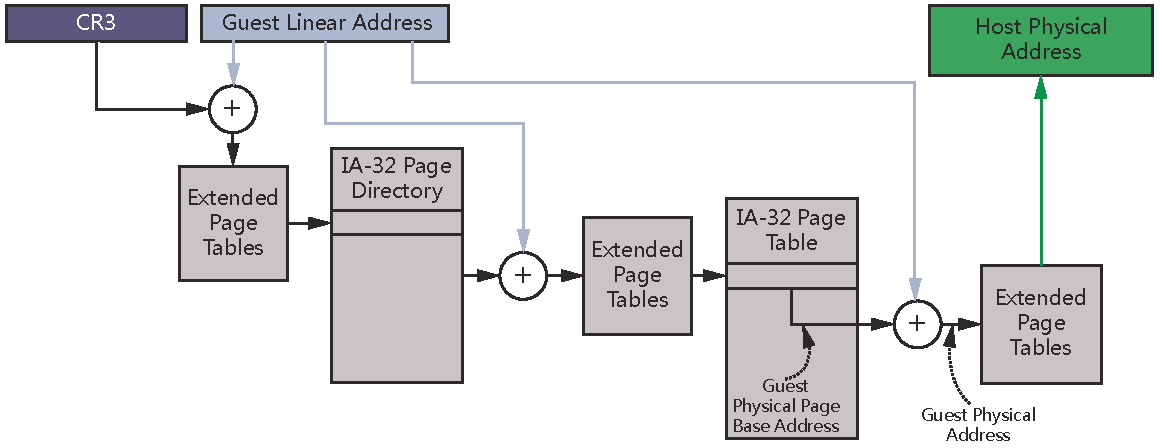
\includegraphics[width=\textwidth]{label/intel-ept-example}
  \caption[Intel Extended Page Table技术示意图]{
    Intel Extended Page Table技术示意图}
  \label{fig:intel-ept-example}
\end{figure}

\textbf{I/O MMU}\quad
IOMMUs are hardware devices that translate
device DMA addresses to proper machine
physical addresses.
which can be used to control how a DMA operation
from a device accesses memory
Intel、AMD和IBM等厂商都提出了自己的I/O MMU方案\cite{intel-iommu, amd-iommu, ibm-iommu},
下文以Intel的I/O MMU为例介绍其功能。

Intel Virtualization Technology for Directed
I/O Architecture provides DMA remapping
hardware that adds support for isolation of device
accesses to memory as well as translation
functionality [2]. The DMA remapping hardware
intercepts device attempts to access system
memory. Then, it uses I/O page tables to
determine whether the access is allowed and
its intended location. The translation structure
is unique to an I/O device function (PCI bus,
device, and function) and is based on a multilevel
page table. Each I/O device is given the
DMA virtual address space same as the physical
address space or a purely virtual address
space defined by software. The DMA remapping
hardware uses a context-entry table that is
indexed by PCI bus, device and function to find
the root of the address translation table. The
hardware may cache context-entries as well as
the effective translations (IOTLB) to minimize
the overhead incurred for fetching them from
memory. DMA remapping faults detected by
the hardware are processed by logging the fault
information and reporting the faults to software
through a fault event (interrupt).



PCI-E标准中使用SR-IOV技术实现I/O设备的共享。

\textbf{Single-Root I/O Virtualization (SR-IOV)}
The Single-Root I/O Virtualization (SR-IOV)
feature is a PCI Special Interest Group (PCISIG)
specification. Intel, along with other
industry leaders, is actively participating in
the PCI-SIG working group to define new
standards for enhancing virtualization capabilities
of I/O devices. SR-IOV provides a
standard mechanism for devices to advertise
their ability to be simultaneously shared
among multiple virtual machines. It also
allows for the partitioning of a PCI function
into many virtual interfaces for the purpose
of sharing the resources of a PCI Express*
(PCIe*) device in a virtual environment. Intel
plans to support the SR-IOV specification in
its networking devices.
Each virtual function can support a unique
and separate data path for I/O-related functions
within the PCIe hierarchy. Use of SRIOV
with a networking device, for example,
allows the bandwidth of a single port (function)
to be partitioned into smaller slices that
may be allocated to specific virtual machines,
or guests, via a standard interface. A common
methodology for configuration and management
is also established to further
enhance the interoperability of various
devices in a PCIe hierarchy. This resource
sharing can increase the total utilization of
any given resource presented on an SR-IOVcapable
PCIe device, potentially reducing the
cost of a virtual system.
Intel-enabled NICs are:
• Intel® 82576 Gigabit Ethernet Controller
• Intel® 82599

\fi

\iffalse
实现多应用的区分化服务,其本质是共享的场景下提供隔离功能,包括资源隔离与性能隔离。
现有技术可以很容易的实现资源隔离,但性能隔离的支持却相对较少。
本节主要介绍现有技术在资源隔离与性能隔离方面的支持,
并讨论引入标签化地址空间实现应用区分的必要性。

\subsection{资源隔离}

从多进程技术出现开始,计算机就开始支持资源隔离,处理器、内存与I/O是主要的需要隔离的资源。
处理器资源的隔离相对比较简单,可以通过处理器核静态分配或基于时间片的调度实现;
地址空间隔离是实现内存资源隔离的主要方式;
而对于I/O资源,普遍在软件层次(如操作系统或Hypervisor/VMM层)实现隔离。
本节将主要对后两种资源的隔离进行讨论。

\textbf{内存资源隔离}\quad	% 进程或虚拟机粒度,通过地址空间隔离实现资源隔离
不同的进程之间具有独立的地址空间,
现代处理器通过内存管理单元(Memory Management Unit,MMU)实现不同进程的地址空间隔离。
处理器核使用虚拟地址进行访问,MMU通过分页或分段机制将虚拟地址转换为物理地址,
操作系统分配并管理MMU使用的地址映射,
将不同进程的虚拟地址空间映射到不同的物理地址空间,实现地址空间的隔离。
以Intel的IA-32/64架构处理器为例,操作系统如Linux仅使用其提供的分页机制,
由内核维护地址映射所需的页表,并通过处理器CR3寄存器将页表地址传递给硬件MMU。
通过以进程为粒度实现地址空间隔离,实现内存资源的隔离。
虚拟化技术出现后,处理器上使用扩展页表(Extended Page Table, EPT)机制,
在原有的两级分页的基础上增加了一级从客户机物理地址(guest-physical address)到
主机物理地址(host-physical address)的映射,
将内存资源隔离的粒度从进程扩大到虚拟机。

\textbf{I/O资源隔离}\quad	% 通过软件在访问端实现隔离
对于I/O资源,操作系统或VMM负责管理整个系统中的I/O设备。
以linux操作系统为例,通过文件的形式为应用提供I/O设备的访问;
而VMM则通过虚拟设备向虚拟机提供I/O设备的访问。
这两种方式都是在软件层次,通过调度的方式实现I/O资源的隔离,
通过共享的操作系统内核或VMM实现对I/O设备访问
从硬件的角度看,

从以上分析可以发现,内存控制器与I/O的资源隔离是在请求源端(处理器)进行的,
通过将不同应用对共享资源的访问划分到不同的位置(内存控制器)或不同的时间(I/O)实现资源隔离。

处理器可以通过调整时间片的长度,实现细粒度的资源隔离;



虽然实现了资源隔离,但在硬件层次并不能支持区分化服务,
对于内存控制器,其收到的请求是直接操作映射后的物理地址,不能区分出应用;
对于I/O设备,其收到的请求已经经过软件层次的仲裁与调试,同样丢失了应用信息。

也正是由于这种应用信息的缺失,在一些共享的硬件部件造成了一定的性能问题,
如虚拟化场景下的TLB和处理器缓存,由于它们不能识别出来自不同虚拟机的请求,
而不同的虚拟机的地址空间的重叠的,因此需要在虚拟机切换时需要无效所有的TLB和处理器缓存,
这带来了极大的性能开销。
为了解决这一问题,Intel在其虚拟化扩展中提出了Virtual Processor IDs(VPID)技术,
通过将虚拟机标识传递到共享的TLB和处理器缓存,
同时在这些共享部件的数据结构中增加了虚拟机标识,
使得在虚拟机切换时只无效必要的表项,降低虚拟机临时切换时重填这些表项的开销。

从以上示例可以发现,实现资源隔离并不需要将应用信息传递到对应的硬件资源上,
但这些应用信息可以用于优化资源隔离的性能。


\subsection{性能隔离}

\fi
